% ------------------------------------------------------------------------
% AMS-LaTeX Paper ********************************************************
% ------------------------------------------------------------------------
% Submitted:      Dec 15 2003
% Final Version:  
% Accepted:       
% ------------------------------------------------------------------------
% This is a journal top-matter template file for use with AMS-LaTeX.
%%%%%%%%%%%%%%%%%%%%%%%%%%%%%%%%%%%%%%%%%%%%%%%%%%%%%%%%%%%%%%%%%%%%%%%%%%

%\documentclass{tran-l}
%\documentclass[twocolumn]{amsart}
%\documentclass[]{amsart}
%\documentclass[]{sig-alternate}
\documentclass[]{acm_proc_article-sp}
%\documentclass[]{llncs}


%\documentclass[]{prentcsmacro}

%\usepackage[active]{srcltx} % SRC Specials for DVI Searching
\usepackage{url}
\usepackage[pdf]{pstricks}
\usepackage{pstricks-add, pst-grad, pst-plot}
\usepackage[tiling]{pst-fill}
\usepackage{verbatim}
\usepackage{graphicx}

\psset{linewidth=0.3pt,dimen=middle}
\psset{xunit=.70cm,yunit=0.70cm}
\psset{angleA=-90,angleB=90,ArrowInside=->,arrowscale=2}


% From Allen's stable.
\usepackage{bigpage}
\usepackage{bcprules}
%\usepackage{code}
\usepackage{mathpartir}
\usepackage{listings}
\usepackage{mathtools}
%\usepackage[fleqn]{amsmath}
\usepackage{amsmath}
\usepackage{amsfonts}
\usepackage{latexsym}
\usepackage{amssymb}
\usepackage{caption}
%\usepackage{multicol}

% Math
\newcommand{\maps}{\colon}
\newcommand{\NN}{\mathbb{N}}
% Double brackets
\newcommand{\ldb}{[\![}
\newcommand{\rdb}{]\!]}
\newcommand{\ldrb}{(\!(}
\newcommand{\rdrb}{)\!)}
\newcommand{\lliftb}{\langle\!|}
\newcommand{\rliftb}{|\!\rangle}
% \newcommand{\lpquote}{\langle}
% \newcommand{\rpquote}{\rangle}
% \newcommand{\lpquote}{\lceil}
% \newcommand{\rpquote}{\rceil}
\newcommand{\lpquote}{\ulcorner}
\newcommand{\rpquote}{\urcorner}
\newcommand{\newkw}{\nu}
\newcommand{\FS}{$\mbox{FinSet}_0$}
\newcommand{\FC}{$\mbox{FinCat}_0$}

% SYNTAX
\newcommand{\id}[1]{\texttt{#1}}
\newcommand{\none}{\emptyset}
\newcommand{\eps}{\epsilon}
\newcommand{\set}[1]{\{#1\}}
\newcommand{\rep}[2]{\id{\{$#1$,$#2$\}}}
\newcommand{\elt}[2]{\id{$#1$[$#2$]}}
\newcommand{\infinity}{$\infty$}

\newcommand{\pzero}{\mathbin{0}}
\newcommand{\seq}{\mathbin{\id{,}}}
\newcommand{\all}{\mathbin{\id{\&}}}
\newcommand{\choice}{\mathbin{\id{|}}}
\newcommand{\altern}{\mathbin{\id{+}}}
\newcommand{\juxtap}{\mathbin{\id{|}}}
%\newcommand{\concat}{\mathbin{.}}
\newcommand{\concat}{\Rightarrow}
\newcommand{\punify}{\mathbin{\id{:=:}}}
\newcommand{\fuse}{\mathbin{\id{=}}}
\newcommand{\scong}{\mathbin{\equiv}}
\newcommand{\nameeq}{\mathbin{\equiv_N}}
\newcommand{\alphaeq}{\mathbin{\equiv_{\alpha}}}
\newcommand{\names}[1]{\mathbin{\mathcal{N}(#1)}}
\newcommand{\freenames}[1]{\mathbin{\mathcal{FN}(#1)}}
\newcommand{\boundnames}[1]{\mathbin{\mathcal{BN}(#1)}}
%\newcommand{\lift}[2]{\texttt{lift} \; #1 \concat #2}
\newcommand{\binpar}[2]{#1 \juxtap #2}
\newcommand{\outputp}[2]{#1 ! ( * #2 )}
\newcommand{\prefix}[3]{#1 ? ( #2 ) \concat #3}
\newcommand{\lift}[2]{#1 ! ( #2 )}
%\newcommand{\quotep}[1]{\lpquote #1 \rpquote}
\newcommand{\quotep}[1]{@#1}
\newcommand{\dropn}[1]{*#1}

\newcommand{\newp}[2]{\id{(}\newkw \; #1 \id{)} #2}
\newcommand{\bangp}[1]{\int #1}
\newcommand{\xbangp}[2]{\int_{#2} #1}
\newcommand{\bangxp}[2]{\int^{#2} #1}

\newcommand{\substp}[2]{\id{\{} \quotep{#1} / \quotep{#2} \id{\}}}
\newcommand{\substn}[2]{\id{\{} #1 / #2 \id{\}}}

\newcommand{\psubstp}[2]{\widehat{\substp{#1}{#2}}}
\newcommand{\psubstn}[2]{\widehat{\substn{#1}{#2}}}

\newcommand{\applyp}[2]{#1 \langle #2 \rangle}
\newcommand{\absp}[2]{\id{(} #1 \id{)} #2}

\newcommand{\transitions}[3]{\mathbin{#1 \stackrel{#2}{\longrightarrow} #3}}
\newcommand{\meaningof}[1]{\ldb #1 \rdb}
\newcommand{\pmeaningof}[1]{\ldb #1 \rdb}
\newcommand{\nmeaningof}[1]{\ldrb #1 \rdrb}

\newcommand{\Proc}{\mathbin{Proc}}
\newcommand{\QProc}{\quotep{\mathbin{Proc}}}

\newcommand{\entailm}{\mathbin{\vdash_{\mathfrak m}}} %matching
\newcommand{\entailp}{\mathbin{\vdash_{\mathfrak p}}} %behavioral
\newcommand{\entailv}{\mathbin{\vdash_{\mathfrak v}}} %validation
\newcommand{\congd}{\mathbin{\equiv_{\mathfrak d}}}
\newcommand{\congs}{\mathbin{\equiv_{\mathfrak s}}}
\newcommand{\congp}{\mathbin{\equiv_{\mathfrak p}}}
%\newcommand{\defneqls}{:\!=}
\newcommand{\defneqls}{\coloneqq}
%\newcommand{\logequiv}{\mathbin{\leftrightarrow}}

\newcommand{\barb}[2]{\mathbin{#1 \downarrow_{#2}}}
\newcommand{\dbarb}[2]{\mathbin{#1 \Downarrow_{#2}}}

% From pi-duce paper
\renewcommand{\red}{\rightarrow}
\newcommand{\wred}{\Rightarrow}
\newcommand{\redhat}{\hat{\longrightarrow}}
\newcommand{\lred}[1]{\stackrel{#1}{\longrightarrow}} %transitions
\newcommand{\wlred}[1]{\stackrel{#1}{\Longrightarrow}}

\newcommand{\opm}[2]{\overline{#1} [ #2 ]} % monadic
\newcommand{\ipm}[2]{{#1} ( #2 )} 
\newcommand{\ipmv}[2]{{#1} ( #2 )} % monadic
\newcommand{\parop}{\;|\;}    % parallel operator
\newcommand{\patmatch}[3]{#2 \in #3 \Rightarrow #1}
\newcommand{\sdot}{\, . \,}    % Space around '.'
\newcommand{\bang}{!\,}
%\newcommand{\fuse}[1]{\langle #1 \rangle}    
\newcommand{\fusion}[2]{#1 = #2} % fusion prefix/action
\newcommand{\rec}[2]{\mbox{\textsf{rec}} \, #1. \, #2}
\newcommand{\match}[2]{\mbox{\textsf{match}} \; #1 \; \mbox{\textsf{with}} \; #2}
\newcommand{\sep}{:}
\newcommand{\val}[2]{\mbox{\textsf{val}} \; #1 \; \mbox{\textsf{as}} \; #2}

\newcommand{\rel}[1]{\;{\mathcal #1}\;} %relation
\newcommand{\bisim}{\stackrel{.}{\sim}_b} %bisimilar
\newcommand{\wb}{\approx_b} %weak bisimilar
\newcommand{\bbisim}{\stackrel{\centerdot}{\sim}} %barbed bisimilar
\newcommand{\wbbisim}{\stackrel{\centerdot}{\approx}} %weak barbed bisimilar
\newcommand{\wbbisimsem}{\approx} %weak barbed bisimilar
\newcommand{\bxless}{\lesssim}  %expansion less (amssymb required)
\newcommand{\bxgtr}{\gtrsim}  %expansion greater (amssymb required)
\newcommand{\beq}{\sim}    %barbed congruent
\newcommand{\fwbeq}{\stackrel{\circ}{\approx}}  %weak barbed congruent
\newcommand{\wbeq}{\approx}  %weak barbed congruent
\newcommand{\sheq}{\simeq}  %symbolic hypereq
\newcommand{\wbc}{\approx_{cb}}

% End piduce contribution

% rho logic

\newcommand{\ptrue}{\mathbin{true}}
\newcommand{\psatisfies}[2]{#1 \models #2}
\newcommand{\pdropf}[1]{\rpquote #1 \lpquote}
\newcommand{\pquotep}[1]{\lpquote #1 \rpquote}
\newcommand{\plift}[2]{#1 ! ( #2 )}
\newcommand{\pprefix}[3]{\langle #1 ? #2 \rangle #3}
\newcommand{\pgfp}[2]{\textsf{rec} \; #1 \mathbin{.} #2}
\newcommand{\pquant}[3]{\forall #1 \mathbin{:} #2 \mathbin{.} #3}
\newcommand{\pquantuntyped}[2]{\forall #1 \mathbin{.} #2}
\newcommand{\riff}{\Leftrightarrow}

\newcommand{\PFormula}{\mathbin{PForm}}
\newcommand{\QFormula}{\mathbin{QForm}}
\newcommand{\PropVar}{\mathbin{\mathcal{V}}}

\newcommand{\typedby}{\mathbin{\:\colon}}
\newcommand{\mixedgroup}[1]{\id{mixed($#1$)}}
\newcommand{\cast}[2]{\id{CAST AS} \; #1 \; (#2)}
\newcommand{\bslsh}{\mathbin{\id{\\}}}
\newcommand{\bslshslsh}{\mathbin{\id{\\\\}}}
\newcommand{\fslsh}{\mathbin{\id{/}}}
\newcommand{\fslshslsh}{\mathbin{\id{//}}}
\newcommand{\bb}[1]{\mbox{#1}}
\newcommand{\bc}{\mathbin{\mathbf{::=}}}
\newcommand{\bm}{\mathbin{\mathbf\mid}}
\newcommand{\be}{\mathbin{=}}
\newcommand{\bd}{\mathbin{\buildrel {\rm \scriptscriptstyle def} \over \be}}
\newcommand{\ctcategory}[1]{\mbox{\bf #1}}

%GRAMMAR
\newlength{\ltext}
\newlength{\lmath}
\newlength{\cmath}
\newlength{\rmath}
\newlength{\rtext}

\settowidth{\ltext}{complex type name}
\settowidth{\lmath}{$xxx$}
\settowidth{\cmath}{$::=$}
\settowidth{\rmath}{\id{attributeGroup}}
\settowidth{\rtext}{repetition of $g$ between $m$ and $n$ times}

\newenvironment{grammar}{
  \[
  \begin{array}{l@{\quad}rcl@{\quad}l}
  \hspace{\ltext} & \hspace{\lmath} & \hspace{\cmath} & \hspace{\rmath} & \hspace{\rtext} \\
}{
  \end{array}\]
}

% Over-full v-boxes on even pages are due to the \v{c} in author's name
\vfuzz2pt % Don't report over-full v-boxes if over-edge is small

% THEOREM Environments ---------------------------------------------------
 \newtheorem{thm}{Theorem}[subsection]
 \newtheorem{cor}[thm]{Corollary}
 \newtheorem{lem}[thm]{Lemma}
 \newtheorem{prop}[thm]{Proposition}
% \theoremstyle{definition}
 \newtheorem{defn}[thm]{Definition}
% \theoremstyle{remark}
 \newtheorem{rem}[thm]{Remark}
 \newtheorem{example}[thm]{Example}
 \numberwithin{equation}{subsection}
% MATH -------------------------------------------------------------------
 \DeclareMathOperator{\RE}{Re}
 \DeclareMathOperator{\IM}{Im}
 \DeclareMathOperator{\ess}{ess}
 \newcommand{\veps}{\varepsilon}
 \newcommand{\To}{\longrightarrow}
 \newcommand{\h}{\mathcal{H}}
 \newcommand{\s}{\mathcal{S}}
 \newcommand{\A}{\mathcal{A}}
 \newcommand{\J}{\mathcal{J}}
 \newcommand{\M}{\mathcal{M}}
 \newcommand{\W}{\mathcal{W}}
 \newcommand{\X}{\mathcal{X}}
 \newcommand{\BOP}{\mathbf{B}}
 \newcommand{\BH}{\mathbf{B}(\mathcal{H})}
 \newcommand{\KH}{\mathcal{K}(\mathcal{H})}
 \newcommand{\Real}{\mathbb{R}}
 \newcommand{\Complex}{\mathbb{C}}
 \newcommand{\Field}{\mathbb{F}}
 \newcommand{\RPlus}{\Real^{+}}
 \renewcommand{\Polar}{\mathcal{P}_{\s}}
 \newcommand{\Poly}{\mathcal{P}(E)}
 \newcommand{\EssD}{\mathcal{D}}
 \newcommand{\Lom}{\mathcal{L}}
 \newcommand{\States}{\mathcal{T}}
 \newcommand{\abs}[1]{\left\vert#1\right\vert}
% \newcommand{\set}[1]{\left\{#1\right\}}
%\newcommand{\seq}[1]{\left<#1\right>}
 \newcommand{\norm}[1]{\left\Vert#1\right\Vert}
 \newcommand{\essnorm}[1]{\norm{#1}_{\ess}}

%%% NAMES
\newcommand{\Names}{{\mathcal N}}
\newcommand{\Channels}{{\sf X}}
\newcommand{\Variables}{{\mathcal V}}
\newcommand{\Enames}{{\mathcal E}}
\newcommand{\Nonterminals}{{\mathcal S}}
\newcommand{\Pnames}{{\mathcal P}}
\newcommand{\Dnames}{{\mathcal D}}
\newcommand{\Types}{{\mathcal T}}

\newcommand{\fcalc}{fusion calculus}
\newcommand{\xcalc}{${\mathfrak x}$-calculus}
\newcommand{\lcalc}{$\lambda$-calculus}
\newcommand{\pic}{$\pi$-calculus}
\newcommand{\rhoc}{${\textsc{rho}}$-calculus}
\newcommand{\hcalc}{highwire calculus}
\newcommand{\dcalc}{data calculus}
%XML should be all caps, not small caps. --cb
%\newcommand{\xml}{\textsc{xml}}
\newcommand{\xml}{XML} 

\newcommand{\papertitle}{Consensus Games}
% use static date to preserve date of actual publication
 \newcommand{\paperversion}{Draft Version 0.1 - 26 August, 2016}

\newenvironment{toc}
{
\begin{list}{}{
   \setlength{\leftmargin}{0.4in}
   \setlength{\rightmargin}{0.6in}
   \setlength{\parskip}{0pt}
 } \item }
{\end{list}}

\newenvironment{narrow}
{
\begin{list}{}{
   \setlength{\leftmargin}{0.4in}
   \setlength{\rightmargin}{0.6in}
 } \item }
{\end{list}}

%%% ----------------------------------------------------------------------

%\title{\huge{\papertitle}}
\title{\papertitle}

%\numberofauthors{3}
\author{
L.G. Meredith\\
  \affaddr{Biosimilarity, LLC}\\
  \email{\fontsize{8}{8}\selectfont lgreg.meredith@biosimilarity.com}
\and
Vlad Zamfir\\
  \affaddr{Ethereum}\\
  \email{\fontsize{8}{8}\selectfont vldzmfr@gmail.com}
\and
Vitalik Buterin\\
  \affaddr{Ethereum}\\
  \email{\fontsize{8}{8}\selectfont vitalik.buterin@ethereum.org}
\and
Matthew Wampler-Doty\\
  \affaddr{MIT}\\
  \email{\fontsize{8}{8}\selectfont matthew.wampler.doty@gmail.com}
\and
Aaron Fisher\\
  \affaddr{Colony}\\
  \email{\fontsize{8}{8}\selectfont aron.mathsguy@gmail.com}
}

%\address{Systems Biology, Harvard Medical School, Boston, Massachussetts, USA}

%\email{lg_meredith@hms.harvard.edu}

%\thanks{This work was completed during a visiting appointment at the Department of Systems Biology, Harvard Medical School.}

%\subjclass{Primary 47A15; Secondary 46A32, 47D20}

%\date{April 6, 2002.}

%\dedicatory{}

%\commby{Daniel J. Rudolph}

%%% ----------------------------------------------------------------------

\begin{document}
%\lstset{language=erlang}
\lstset{language=}

%These margin values appear to be relative to the bigpage package settings. --cb
\setlength{\topmargin}{0in}
\setlength{\textheight}{8.5in}
\setlength{\parskip}{6pt}

\keywords{ consensus, games semantics, concurrency, message-passing, types, Curry-Howard }

\begin{abstract}
\normalsize{ 

  We present an axiomatic framework for reasoning about consensus protocols.

}

\end{abstract}

% \noindent
% {\large \textbf{Submission to arXiv}}\\
% \rule{6.25in}{0.75pt}\\\\\\

%%% ----------------------------------------------------------------------
\maketitle
%%% ----------------------------------------------------------------------

% \begin{center}
% \paperversion\\
% \end{center}

% \begin{toc}
% \tableofcontents
% \end{toc}

% \newpage
% ------------------------------------------------------------------------

\section{Introduction and motivation}

Our aim is to describe an axiomatic framework for analyzing and
comparing a wide range of consensus protocols. The intended outcome is
a proof of the safety and termination properties of class of consensus
protocols, under a wide class of fault and network conditions.

\subsection{Related work}

This work builds on several strands of research. One of the main
strands is the line of investigation begun by Linear Types Can Change
The Blockchain (pdf, lex, hangout video) . Another strand is the
seminal work by Vlad Zamfir and Vitalik Buterin on Casper. Another
strand of research is the work on games semantics for programs
initiated by Abramsky, Hyland, and Ong.

\subsection{Outline of paper}

First we set out the basic elements and intuitions of the technical
framework. Then we build up a compositional model of typed consensus
protocols in which types describe safety and liveness properties.

\section{Technical framework}

Consensus games take place amongst a set, P, of players who are
concurrently sending messages to each other. Each message is an
announcement of a position in the game, which we dub here a bet,
indicating a player's belief in a claim that the players will agree on
a value v at the conclusion of the game. Bets are described by the
following recursive domain equation.

\subsection{Bets}

\begin{defn}[Bet] \label{def.bet}
  \begin{equation*}
    \begin{aligned}
      B[P,C,F] = 1 + P \times P \times C \times F \times \mathsf{List}[B[P,C,F]]
    \end{aligned}
  \end{equation*}
\end{defn}
  
Recall the equation for n-ary $A$-labelled trees is given by

\begin{equation*}
  \begin{aligned}
    \mathsf{Tree}[A] = 1 + A \times \mathsf{List}[Tree[A]]
  \end{aligned}
\end{equation*}
    
and note that $B[P,C,F] = \mathsf{Tree}[P \times P \times C \times F]$

In the sequel we will let $b$, $b'$, etc range over bets and for
convenience, we give logical accessors to components of the bet via
the projections, $\pi_i$. Following executable specification
languages like Haskell or Scala, we can improve readability 

\begin{equation*}
  \begin{aligned}
    \mathsf{src}( \mathsf{inr}( ( s, t, c, f, j ) ) = s  \\
    \mathsf{trgt}( \mathsf{inr}( ( s, t, c, f, j ) ) = t \\
    \mathsf{claim}( \mathsf{inr}( ( s, t, c, f, j ) ) = c  \\    
    \mathsf{belief}( \mathsf{inr}( ( s, t, c, f, j ) ) = f  \\    
    \mathsf{justify}( \mathsf{inr}( ( s, t, c, f, j ) ) = j 
  \end{aligned}
\end{equation*}

We understand these components of the data structure to have the
following meaning

\begin{itemize}
  \item $\mathsf{src}( b )$ represents the source or origin of the
    bet, i.e. the player who is sending the bet;
  \item $\mathsf{trgt}( b )$ represents the target or destination of
    the bet message, i.e. the player who is the intended recipient of
    the bet;
  \item $\mathsf{claim}( b )$ represents the claim of the bet,
    i.e. the source player's estimate of a value;
  \item $\mathsf{belief}( b )$ represents the source player's confidence in
    the claim given the evidence in the justification;
  \item $\mathsf{justify}( b )$ represents the justification or
    evidence of the claim or estimate made in the bet
\end{itemize}

\subsubsection{Temporal order} 

Notice that there is an implicit description
of time in the bet data structure in the sense that the justification
of a bet contains the history of observations leading up to that bet;
and this can be formalized by

\begin{defn}[Temporal order]
  \begin{equation*}
    \begin{aligned}
      b_1 \sqsupseteq b_2 \iff b_2 \in \mathsf{justify}(b_1) or \exists b_3 \in \mathsf{justify}(b_1). b_3 \sqsupseteq b_2    
    \end{aligned}
  \end{equation*}
\end{defn}

From this perspective the choice of whether the collection of bets in
the justification of a particular bet, say $b$, is a ordered
($\mathsf{List}$) as in definition \ref{def.bet} or unordered
($\mathsf{Set}$) correlates to whether history is totally ordered or
partially ordered. When the justification is ordered, the temporal
order relation can by made total using the order of the justification
together with the ordering of the tree. When interpreting bets as
messages in a message-passing protocol, the choice of an unordered
justification can be used to represent message arrival order
non-determinism.

\subsubsection{Visualizing bets}

The data structure allows to recover a great deal of information about
network communication. To see this, let's consider the following
example.

\begin{figure}
  \begin{center}
    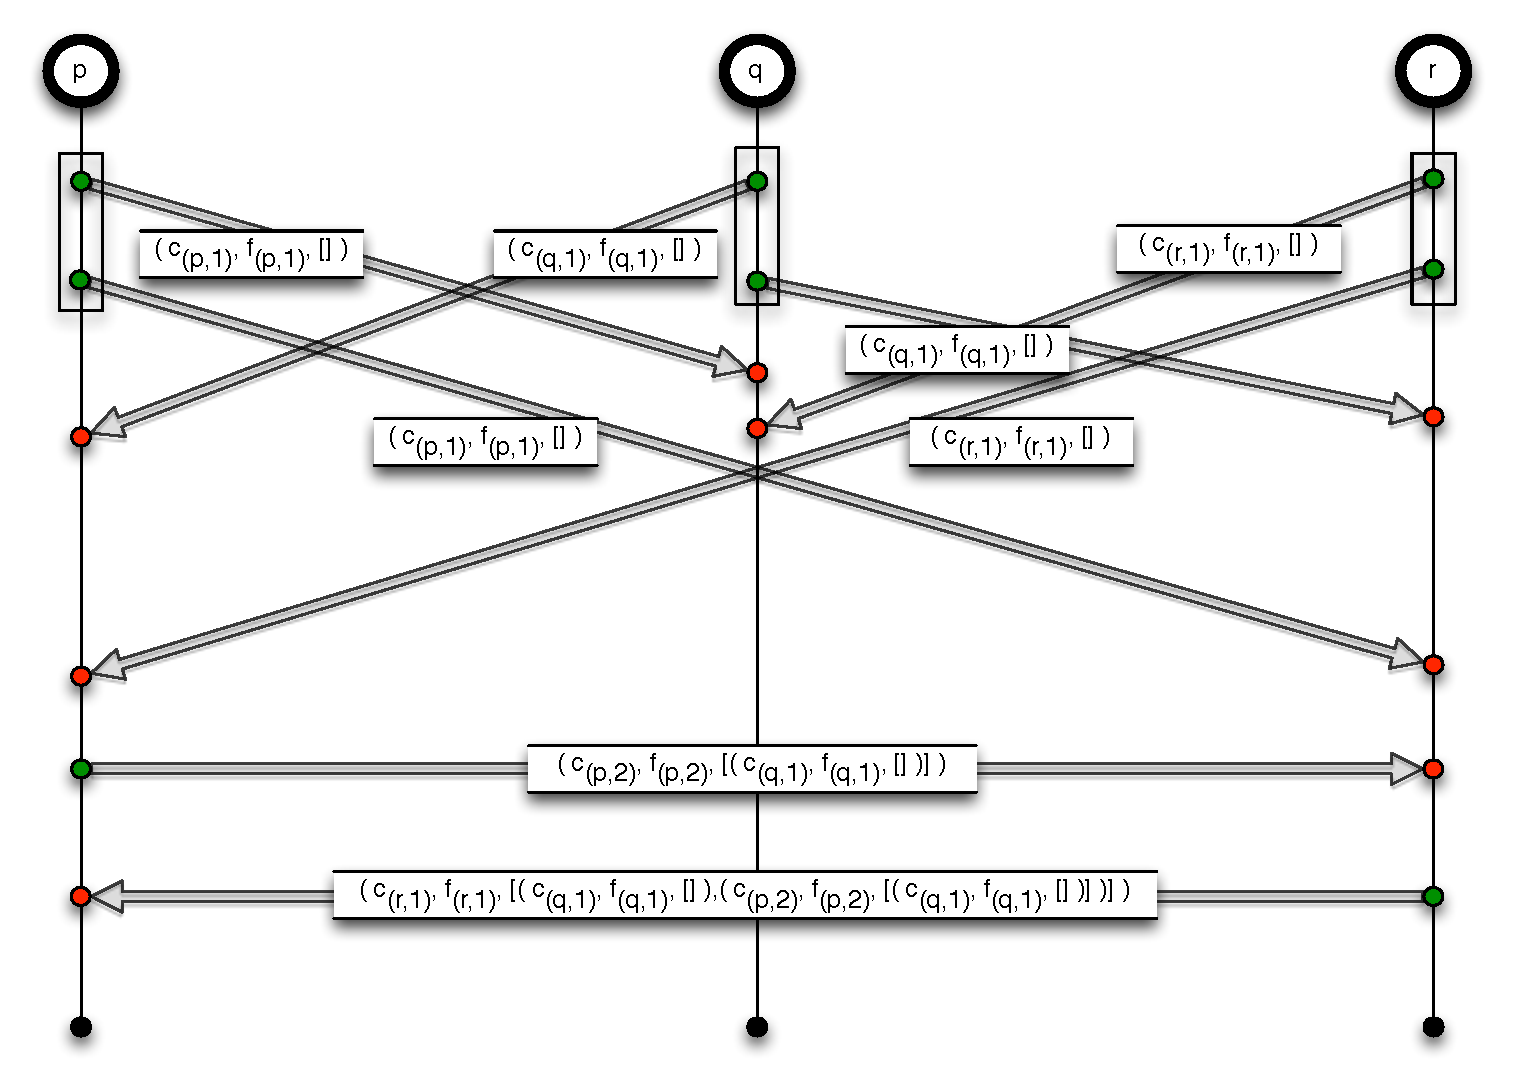
\includegraphics [width=\linewidth,keepaspectratio]{/Users/luciusmeredith/work/src/projex/stellar/mdp4tw/Synereo/pi4u/cg/ConsensusGamesDiagram1.pdf}
    \caption{Non-redundant bet}
    \label{redundant-bets}
  \end{center}
\end{figure}

\begin{equation*}
  \begin{aligned}[l]
    b_{p \to q/1} = inr( ( p, q, c_{(p,1)}, f_{(p,1)}, [] ) ) \\
    b_{p \to r/1} = inr( ( p, r, c_{(p,1)}, f_{(p,1)}, [] ) ) \\
    b_{q \to p/1} = inr( ( q, p, c_{(q,1)}, f_{(q,1)}, [] ) ) \\
    b_{q \to r/1} = inr( ( q, r, c_{(q,1)}, f_{(q,1)}, [] ) ) \\
    b_{r \to p/1} = inr( ( r, p, c_{(r,1)}, f_{(r,1)}, [] ) ) \\
    b_{r \to q/1} = inr( ( r, q, c_{(r,1)}, f_{(r,1)}, [] ) ) \\
    b_{p \to r/2} = inr( ( p, r, c_{(p,2)}, f_{(p,2)}, [b_{q \to p/1}] ) ) \\
    b_{r \to p/2} = inr( ( p, r, c_{(p,2)}, f_{(p,2)}, [b_{q \to r/1},b_{p \to r/2}] ) ) \\
  \end{aligned}
\end{equation*}

This collection of bets can be visualized as an \emph{interaction
  diagram} amongst the players, $p,q$, and $r$ as depicted in figure
\ref{redundant-bets}. Time runs from top to bottom. Arrows indicate
the communication of bets, with source and target information depicted
by both the arrow orientation and the green and red vertices. The
latter provides a visual aid to readily identify the view a particular
player has of the network at any given time. Specifically, a player's
view at a given time is simply the collection of red vertices up to
the depth corresponding to that time. In a somewhat non-standard way,
we use rectangular boxes around vertices to indicate concurrency, or
no ordering on particular communication events. Thus, for example,
$b_{p \to q/1}$ and $b_{p \to r/1}$ are indicated as sent in parallel. It
is only $q$'s view of events that determines their arrival order for
$q$.

\subsubsection{Information density}

The specification for bets allows for a wide range of structures that
are not necessarily ideal message structures. Consider the following
bet extending the example above.

\begin{equation*}
  \begin{aligned}[l]
    b_{p \to r/3} = inr( ( p, r, c_{(p,3)}, f_{(p,3)}, [b_{q \to p/1},b_{r \to p/2}] ) )
  \end{aligned}
\end{equation*}

Because $b_{r \to p/2}$ already includes $b_{q \to p/1}$, indicating
that $r$ has already seen $p$'s evidence for what it has seen from
$q$, and that $p$ was the provider of said evidence, including this
evidence is clearly redundant. While redundancy can be beneficial in
certain contexts, it is generally harmful here, providing an overhead
on communication that can be used maliciously. So, we want to restrict
our attention to redundancy-free bets. Notice, however, that the
notion is somewhat subtle. For example, even though $b_{p \to r /2}$
includes $b_{q \to r/1}$, the justification of $b_{r \to p/2}$ cannot be
considered redundant because it provides potentially useful
information about the arrival order of bets at $r$.

We can formalize the notion of redundancy-free bets using a notion of
path. Since a bet is really just a labelled n-ary tree, we can talk
about paths in a bet, which are simply sequences of bets,
i.e. elements of $\mathsf{List}[B[P,C,F]]$. We denote the set of paths
from $b$ with $\mathsf{paths}(b)$ and use $\sigma$ to range
over $\mathsf{paths}(b)$, $|\sigma|$ to denote the length of $\sigma$ and
0-based indexing notation to denote positions in the path. Thus, for
example, $\sigma(0)$ is the initial bet in the path, and $\sigma(
|\sigma| - 1)$ denotes the final bet in the path.

\begin{defn}[redundancy-free]
  A bet, $b$, is redundancy-free iff
  \begin{flalign*}
    b' \in \mathsf{justify}( b ) & \Rightarrow \\
    & \forall \sigma \in List[B[P, C,F]]. \\
    & \;\;\;\;\sigma( 0 ) \in \mathsf{justify}( b ) \;\&\; src( \sigma( | \sigma | - 1 ) ) = src( b ) \\
    & \;\;\;\;\Rightarrow b’ \notin \mathsf{justify}( \sigma( | \sigma | - 1 ) )
  \end{flalign*}
\end{defn}

\subsection{Strategies}

A consensus game is determined, in part, by a move relation, $\vdash$,
on pairs of sets of bets, $( M, N ) \in \mathcal{P}( B[P,C,F] ) \times
\mathcal{P}( B[P,C,F] )$ indicating the legal moves. The statement $M
\vdash N$ indicates that given the set of bets $M$, a player who plays
by the rules produces a bet in $N$.

\begin{defn}[strategy]
  A strategy, $s$, is a map $s : \mathcal{P}( B[P,C,F] ) \to B[P,C,F]$, that produces
  a new bet from the information contained in a set of bets given as
  arguments to $s$. We use $S$ to range over sets of strategies, that is,
  $S \subseteq \mathcal{P}( B[P,C,F] ) \to B[P,C,F]$.
\end{defn}

\begin{defn}
  A strategy, $s$, is said to be legal w.r.t $\vdash$, alternatively, $\vdash$-legal,
  iff

  $M \subseteq B[P,C,F] \To \exists N \subseteq B[P,C,F]. s( M ) \in N \&  M \vdash N$.
\end{defn}

In the sequel we will want to associate players with strategies, and
use $S$ to range over the set of partial maps $P \Rightarrow ( \mathcal{P}( B[P,C,F] ) \Rightarrow B[P,C,F] + 1 )$.

\subsection{Relationship to traditional notions of consensus}

Roughly speaking, a consensus protocol implies a legal move
relation. N.b. illegal moves are evidence of Byzantine
behavior. Traditionally, a consensus protocol also implies a strategy,
and Byzantine behaviour in the canonical consensus literature includes
playing any strategy that isn’t “protocol”. The framework of
definitions above is more relaxed. There will be legal strategies that
would be considered Byzantine in traditional consensus literature. For
example, a Byzantine node, in the classical consensus literature,
could delay publishing bets without making any illegal moves.

\subsection{Games}

We capture the dynamics of game play through the notion of a history of a game. 

\begin{defn}
  Given a move relation and a set of players, $P$, we can describe a
  complete game history $H$ as a partial map
  \begin{flalign*}
    H : P \times \mathcal{List}[\mathcal{Set}[B[P,C,F]] + \mathcal{Set}[B[P,C,F]]] \\
    & \to \mathcal{Set}[B[P,C,F]] + \mathcal{Set}[B[P,C,F]] + 1
  \end{flalign*}
  \begin{itemize}
    \item $H( p, l ) \mapsto \mathcal{inr}( A' )$ indicates that $A'$ is the last set of bets p will see in this history, while
    \item $H( p, l ) \mapsto \mathcal{inl}( A' )$ indicates that $p$ will receive bets after $A'$
    \item $H( p, l ) \mapsto \bot$ indicates that $H$ is undefined, i.e. that $p$ will never see $l$ and so cannot see an extension of $l$.
  \end{itemize}
\end{defn}

\begin{defn}
  We define the $H$-messages of $l$ for $p$ from $p'$, $msgH( l, p, p’ )$, as

  \begin{equation*}
    msgH( l, p, p' ) = trgt( H( p', l ), p )
  \end{equation*}
\end{defn}

This is under ideal network conditions where all messages sent
arrive. It will be convenient to address network conditions separately
from the choices of players to send messages. For this we will adopt a
notation $msgH( l, p, p’; C )$, which we detail in a separate section.

%% Defn. We define the H-extension of l for p, extH( l, p ) as

%% extH( l, p ) = ∪p’≠p msgH( l, p, p’ )

%% The next definition derives from the style of defining streams lazily from generators. For example, we can define the stream of counting numbers [ 0, 1, 2, … ] by

%% N = 0 :: map( λn.n + 1, N )

%% Defn. We define the H-stream, alternatively H-view, of p, H( p ), as

%% H( p ) = map( λn. if 0?( n ) then [] else let l = take(n, H( p ) ) in l :: [ extH( p, l ) ], N )

%% Defn. Given a map, S, taking players to their strategies, we say that H respects S at l iff for all p ∈ P, A ∈ msgH( l, S( p ) ), src( A, S( p’ ) ) ⊆ S( p’ )( l ). Likewise, H respects S iff for all p ∈ P, l ∈ H( s ), H respects S at l.

%% Defn. Given a map, S, taking players to their strategies, we say that H is S-continuous iff
%% exists n.H( S( p ) )( n ) match inr( A ) implies for all n’ > n H( S( p ) )( n’ ) = ⊥
%% H respects S.

%% Notice that this describes an actual history of message passing amongst the players, rather than enumerating possible plays. As long as we remain aware of the distinction between actual histories and possible histories, we can identify a game with a triple, G = ( S,  ⊢, H ), consisting of a map of players to strategies, S, a legal move relation, ⊢, and an S-continuous H; and as before avail ourselves of logical accessors, SG, ⊢G, HG, denoting the components of G, respectively.

%% Defn. We say a set of bets, A ⊆ B[P,C,F], agrees on a value, v, and write A⇓v, when A = claim( A, v ).

%% Defn. A game, G, computes a value, v, written G⇓v, when there is a set, A ⊆ B[P,C,F]), such that A⇓v and for each legal strategy s ∈ SG and A’ ⊆ A, s( A’ ) ∈ A. That is, A agrees on v, and is an attractor for the iterated function system generated by the legal strategies of SG. When G⇓v write attractor( G, v ) for A.

%% Thm. G⇓v iff 
%% for all p such that S( p ) is ⊢-legal there exists l such that H( p, l )⇓v
%% ∪l ∈ { l | H( p, l )⇓v } H( p, l ) ⊆ attractor( G, v )
%% Pf. Immediate.

%% Intuitively, when a game computes a value, it represents message passing behavior amongst the players that results in consensus on the value. However, it is important to note that games, as defined, here, involve actual histories of message-passing behavior. They are a record or trace of a “machine” built out of message-passing behavior over a collection of agents. As such, the current description does not account for partial or incomplete knowledge which may represent the individual views of the players during the state of play, or of “clients” of this machine.

\subsection{Composition of games}

\section{Formulae}

\section{Safety and liveness}

\section{Conclusions and future work}

TBD

\paragraph{Acknowledgments}

TBD

% ------------------------------------------------------------------------
%GATHER{Xbib.bib}   % For Gather Purpose Only
%GATHER{Paper.bbl}  % For Gather Purpose Only
\bibliographystyle{amsplain}
\bibliography{cg}

% ------------------------------------------------------------------------



% ------------------------------------------------------------------------

\end{document}
% ------------------------------------------------------------------------
